% !TeX encoding = UTF-8
% !TeX TXS-program:compile = txs:///latexmk/{-pdf} -xelatex
% !TeX TXS-program:recompile-bibliography = txs:///latexmk/{} -v

% 载入 SJTUThesis 模版
\documentclass[type=bachelor,oneside,openany]{sjtuthesis}
% 选项
%   type=[doctor|master|bachelor],     % 可选（默认：master），论文类型
%   zihao=[-4|5],                      % 可选（默认：-4），正文字号大小
%   lang=[zh|en|de|ja],                % 可选（默认：zh），论文的主要语言
%   review,                            % 可选（默认：关闭），盲审模式
%   [twoside|oneside],                 % 可选（默认：twoside），双页或单页边距模式
%   [openright|openany],               % 可选（默认：openright），奇数页或任意页开始新章
%   math-style=[ISO|TeX],              % 可选 (默认：ISO)，数学符号样式
%   preset=[base|jwc],                 % 可选（默认：base），预设配置，学士学位论文考虑使用 jwc 预设

% 论文基本配置，加载宏包等全局配置
\input{setup}

\begin{document}

%TC:ignore

% 标题页
\maketitle

% 原创性声明及使用授权书
\copyrightpage
% 插入外置原创性声明及使用授权书
% 此时必须在导言区使用 \usepackage{pdfpages}
% \copyrightpage[file=scans/sample-copyright-a.pdf]

% 前置部分
\frontmatter

% 摘要
% !TEX root = ../main.tex

\begin{abstract}[zh]
  随着区块链生态的持续发展，单一区块链系统已经难以满足多链资产流通、跨平台业务协作和异构链互操作的需求。除了在跨链代币转移过程中公证人（Notary）的资产抵押需求影响了跨链流通性之外，不同区块链在账户模型、共识机制、智能合约能力、交易确认方式以及脚本表达能力方面存在明显差异，使得资产无法像同一系统内部转账一样直接从一条链迁移到另一条链。因此，通过区块链互操作算法和协议的研究，解决在异构区块链之间的跨链资产交换成为区块链技术演进的关键挑战之一。跨链协议不仅需要完成源链与目标链之间的状态协调，还需要保证交易过程中的原子性、安全性和失败回滚能力，避免出现一方资产已经锁定或支付，而另一方无法获得对应资产的情况。

  针对上述问题，本文设计并实现了一个基于公证人协调与哈希时间锁的跨链资产交换原型系统。系统采用 Alice - ManagerA - Notary - ManagerB - Bob 的角色协作模型，其中 Alice和Bob 分别作为跨链交易的发起方和目标链接收方，ManagerA 与 ManagerB 分别负责源链和目标链上的资产池管理，Notary 作为公证与中继节点负责监听链上事件并协调目标链响应。在支持智能合约的链上，系统通过 HTLC 哈希时间锁机制实现资产锁定、条件领取和超时退款；针对 Monero、ZCash 屏蔽交易等不具备通用脚本能力的无脚本链，由于 HTLC 所依赖的哈希锁判断和条件分支逻辑无法在链上表达，系统引入 Schnorr adaptor signature，将锁定条件从脚本层转移到签名补全过程，使条件化交易在仅具备签名能力的链上同样可以实现，解决了异构跨链的原子性和安全问题。原型实现以 BTC 作为 scriptless 场景的替代实现，用于验证 adaptor signature 机制在签名补全与秘密提取上的正确性。本文围绕系统架构、核心机制、合约实现、公证人协调流程、scriptless 适配方式、安全性分析以及实验展示进行论述，证明该原型系统能够在统一跨链流程下兼容从智能合约链到无脚本链的不同执行能力，为多种异构链之间的资产交换提供可靠、高效的解决方案。

\end{abstract}

\begin{abstract}[en]
  This thesis designs and implements a cross-chain asset exchange prototype based on notary coordination and hashed timelock contracts. The system follows the role model of Alice, ManagerA, Notary, ManagerB, and Bob. For contract-capable blockchains, the system uses HTLCs to express asset locking, conditional claiming, and timeout refunding on chain. For scriptless blockchains such as Monero and ZCash shielded transactions, where the hash-lock checks and conditional branches required by HTLCs cannot be expressed on chain, the system introduces Schnorr adaptor signatures to move the locking condition from the script layer into the signature adaptation process, so that conditional transactions remain achievable on chains that only support signing. The prototype uses Bitcoin as a stand-in for the scriptless scenario to validate the correctness of the adaptor signature mechanism in signature completion and secret extraction. The thesis presents the system architecture, core mechanisms, implementation modules, security analysis, and experimental validation, showing that the prototype can provide a unified workflow for heterogeneous blockchain asset exchange ranging from smart-contract chains to scriptless chains.
\end{abstract}


% 目录
\tableofcontents
% 如需插图索引、表格索引或符号表，可在后续定稿时启用。
% \listoffigures
% \listoftables
% \listofalgorithms
% \input{contents/nomenclature}

%TC:endignore

% 主体部分
\mainmatter

% 正文内容
% !TEX root = ../main.tex

\chapter{绪论}

\section{研究背景：跨链资产交换}

区块链技术通过分布式账本、密码学签名和共识机制实现了去中心化的价值记录与转移~\cite{nakamoto2008bitcoin,zheng2018blockchain}。随着以太坊、比特币、BSC、Conflux 等公链以及 Hyperledger Fabric 等联盟链的发展，区块链逐渐形成公链与联盟链并存的多链生态格局~\cite{lohachab2021towards}。不同形式和技术的区块链基于其在共识性能、节点组织形式上的不同，适用的应用场景具有显著差异。比如，以Etheruem, Conflux等区块链基于他们强大的合约虚拟环境和庞大的节点支持，在面向以智能合约执行的分布式业务中具有显著优势；而联盟链基于其相比公有链更高的交易吞吐率，侧重高性能交易处理；另外，以门罗币，零币为代表的区块链通过密码手段代替脚本机制，则为以安全性和价值保护为核心目标的业务提供极高的安全保障。
需要强调的是，门罗币（Monero）、Zcash 等无脚本/强隐私区块链同样存在明确的跨链互通诉求，而非孤立于多链生态之外。其核心矛盾在于：隐私币用户既希望保有链上隐私与资产安全，又需要在不依赖中心化托管交易所的前提下，将隐私资产兑换为比特币、以太坊等主流资产，或反向完成入金；若只能通过中心化平台出入金，则会重新引入托管风险并削弱隐私设计初衷。Thyagarajan 等人提出的 Universal Atomic Swaps 指出，Monero、Zcash 屏蔽地址以及 Mimblewimble 等系统因不支持哈希锁与时间锁脚本，传统 HTLC 原子交换无法直接适用，因而需要仅依赖签名验证能力的通用跨链方案~\cite{thyagarajan2022universal}。面向门罗币，Thyagarajan、Malavolta 等人进一步提出 PayMo，基于可验证定时可链接环签名构造与门罗币交易格式兼容的无脚本原子交换，使其可与比特币、以太坊等多种主流币种安全互换~\cite{thyagarajan2022paymo}；Hoenisch 等人提出的 LightSwap 则给出比特币与门罗币之间的轻量原子交换协议，说明该类互通具备可落地的工程场景~\cite{hoenisch2022lightswap}。针对 Zcash，Sanchez 等人提出 Bridging Sapling（ZCLAIM），面向 Sapling 屏蔽池设计隐私跨链资产迁移框架，表明隐私币用户同样需要在尽量保持隐私的同时完成跨链资产流转~\cite{sanchez2022zclaim}。Han 等人提出的 P2C2T 进一步指出，异构货币系统间缺乏同时满足原子性、隐私性与实用性的互联机制，并给出仅要求底层链具备签名验证能力的隐私跨链转移方案~\cite{han2025p2c2t}。综上，无脚本隐私链的跨链诉求可概括为三点：去中心化兑换与出入金、与主流链资产互通而不破坏隐私/可互换性，以及在脚本能力缺失条件下仍能完成原子交换。
然而，多链生态也带来了资产和状态割裂的问题~\cite{JSGG202402003}。某一条链上的账户余额、交易记录和合约状态通常不能被另一条链直接读取或修改，用户如果希望在不同链之间完成资产交换，不能简单地调用一次普通转账交易，而必须借助跨链协议完成多链状态协调~\cite{zamyatin2021sok}。

跨链资产交换的本质并不是把同一个资产实体从一条链物理搬运到另一条链，而是在两个相互独立的账本系统之间建立可信的价值对应关系。以 Alice 与 Bob 的交换为例，Alice 希望在源链上支付一定数量的资产，Bob 在目标链上收到等值资产。由于两条链的交易确认相互独立，如果没有额外机制，Alice 支付后 Bob 可能无法收到资产，或者 Bob 收到资产后 Alice 的支付无法完成。跨链系统必须解决”谁先执行””如何证明对方已执行””失败后如何回滚”等核心问题。

在传统中心化交易平台中，这类问题通常由平台托管资产并撮合交易解决，但这种方式引入了中心化信任风险。平台一旦出现作恶、被攻击、运营失败或提现限制，用户资产可能遭受损失。去中心化跨链交换希望通过链上合约、密码学锁定、事件监听和中继机制降低对单一中心化实体的依赖，使资产释放条件由可验证的协议规则控制~\cite{zamyatin2021sok}。本文所研究的系统正是面向这一问题的原型实现，旨在通过多角色协作和密码学条件锁定，为跨链资产交换提供一种结构清晰、安全可分析的设计方案。

\section{研究意义}

跨链资产交换的研究具有较强的现实意义和工程价值。从需求侧看，多链生态已经成为区块链应用发展的常态~\cite{JSGG202402003,lohachab2021towards}，用户希望将一条链上的原生资产转换为另一条链上的资产，或者在不同链之间使用同一套应用服务。如果缺少跨链能力，各链将形成相互割裂的价值孤岛，限制区块链应用的扩展和用户体验的统一。

从技术方案看，现有跨链方案大致可分为中继链验证、侧链/桥托管和原子交换三类~\cite{Zhu2024,3845}。中继链验证安全性较强但实现成本高，对链的合约能力和验证能力要求较高，Cosmos~\cite{kwon2019cosmos} 和 Polkadot~\cite{wood2016polkadot} 是这一方向的典型代表；侧链/桥托管实现相对简单但引入了中心化信任假设~\cite{back2014enabling,singh2020sidechain}，削弱了区块链系统本身强调的去中心化特性。基于 HTLC 的原子交换~\cite{10.1145/3212734.3212736} 提供了一种较轻量的折中方案，通过 hashLock 和 timeLock 将两侧资产的领取条件绑定在同一个 secret 上，能够在不完全信任对手方的情况下完成交换~\cite{poon2016bitcoin}，同时结合公证人协调机制~\cite{xiong2022notary,9860209} 可以兼顾流程自动化与安全性。

与部分依赖流动性提供者或中继节点在目标链垫付资产的跨链桥不同~\cite{yin2022bool}，本文将 Notary 限定为事件监听和消息协调角色。Notary 不承担资产托管或目标链流动性提供职责，其主要作用是观察源链事件、解析跨链参数并推动目标链创建对应锁定。资金锁定和释放由两侧 Manager/TokenPool 以及 HTLC 或 adaptor signature 条件机制约束。换言之，Notary 在真实链上仍需要承担提交交易所需的 gas 成本，但不需要为用户跨链交换提供目标链资产流动性，这有助于降低中继节点的资金门槛，并使系统安全性更多依赖可验证的合约条件和密码学关系。

从技术难点看，异构链兼容是跨链系统必须面对的挑战。不同链在脚本表达能力上差异巨大：EVM 类链可以直接部署智能合约，通过合约状态记录 hashLock、timeLock、swapId 和资产锁定情况，HTLC 所需的哈希锁判断和条件分支都能在链上显式表达；而 Monero、ZCash 屏蔽交易等无脚本链以纯密码学方式构造交易，不提供通用脚本能力，HTLC 依赖的链上条件逻辑根本无法迁移~\cite{9833731}。相关工作也从应用侧印证了这一缺口：Thyagarajan 等人~\cite{thyagarajan2022universal} 与 Han 等人~\cite{han2025p2c2t} 均将“仅依赖签名验证”作为覆盖隐私币与异构账本的最小能力假设；Thyagarajan 等人~\cite{thyagarajan2022paymo}、Hoenisch 等人~\cite{hoenisch2022lightswap} 与 Sanchez 等人~\cite{sanchez2022zclaim} 的研究则分别表明，门罗币与 Zcash 用户需要在不硬分叉、尽量保持隐私与可互换性的前提下完成与比特币等链的原子交换或资产迁移。如果跨链系统只支持一种合约模型，就无法覆盖这一类只能签名、不能执行脚本的链。本文将 HTLC 与 Schnorr adaptor signature~\cite{9833731} 放在统一跨链架构下讨论：对于合约能力较强的链使用链上 HTLC，对于无脚本链则将条件锁定逻辑放入签名补全过程中，使条件化交易在仅具备签名能力的链上同样能够实现，从而在统一流程下覆盖从智能合约链到无脚本链的不同执行能力。

除了算法理论层面提出跨链资产交换协议之外，本文同样开发了能在主流区块链系统间真实跨链转账的原型系统，具有系统实现方面的重要意义。项目中包含 Solidity 智能合约、Python 后端协调服务、scriptless 场景下的 adaptor signature 模拟模块（以 BTC 作为替代实现）和前端可视化页面，能够较完整地展示跨链资产交换从协议设计到代码实现再到流程演示的全过程。

\section{本文主要工作}

本文围绕跨链资产交换原型系统，从架构设计、核心机制实现和安全性分析三个层面展开工作。

在架构设计层面，本文提出了 Alice - ManagerA - Notary - ManagerB - Bob 的跨链角色模型。该模型将用户、资金池管理者、公证中继节点和目标链接收方明确区分，使系统能够清晰表达资产控制边界与消息协调之间的关系，避免将跨链流程简单等同于单个合约调用。系统将跨链资产交换拆分为用户发起、资金池锁定、事件监听、目标链响应、秘密揭示、资产释放与超时退款等阶段，每个阶段由对应角色驱动。

在核心机制实现层面，本文针对不同链的脚本表达能力设计了两种条件锁定方式。对于支持智能合约的链，系统通过 HTLC 实现资产锁定，使用 hashLock 约束领取条件、timeLock 约束退款条件、swapId 关联同一笔跨链请求，形成源链与目标链的状态配对。对于 Monero、ZCash 屏蔽交易等无脚本链，由于 HTLC 所需的哈希锁判断和条件分支无法在链上表达，系统引入 Schnorr adaptor signature，将完成条件嵌入签名补全过程，以纯密码学方式实现条件化交易，使这类只能签名、不能执行脚本的链也能参与跨链原子交换。在两种机制之上，Notary 作为公证人监听源链合约事件，读取跨链参数并协调目标链 Manager 创建对应锁定，承担跨链消息传递和流程推动的职责。工程实现方面，智能合约模块负责资产池和 HTLC 状态管理，Python 后端模块负责跨链协调，前端模块用于展示跨链流程中各角色状态、密码学参数和交易进度的变化。

在安全性分析层面，本文对系统的原子性、可退款性、Notary 信任边界、Manager 约束和异构兼容能力进行了讨论，说明该系统在原型层面能够满足跨链资产交换的基本安全要求。

本文其余部分组织如下：第二章介绍 HTLC 和 Schnorr adaptor signature 的相关技术背景；第三章阐述系统总体设计，包括角色模型、模块划分和跨链流程；第四章详细描述核心机制的设计与实现；第五章进行系统安全性分析；第六章展示系统实现与实验验证；第七章总结全文并讨论后续工作方向。


% !TEX root = ../main.tex

\chapter{相关技术}


\section{HTLC 哈希时间锁}


HTLC 全称为 Hashed TimeLock Contract，即哈希时间锁合约~\cite{poon2016bitcoin,10.1145/3212734.3212736}。它被广泛应用于链下支付通道和跨链原子交换中。其核心思想是将资产领取条件拆分为两个部分：哈希锁和时间锁。哈希锁要求领取方必须提交一个 secret，使得该 secret 经过哈希计算后等于合约中预先保存的 hashLock；时间锁则规定如果在指定时间内没有人提交正确 secret，资产可以被原始锁定方取回。


HTLC 的基本流程可以描述为：Alice 首先生成随机 secret，并计算 hashLock = H(secret)。在发起跨链交换时，Alice 并不公开 secret，而是将 hashLock 写入源链锁定合约。目标链也使用同一个 hashLock 创建对应锁定。这样，两条链上的资产虽然位于不同账本中，但它们的领取条件都被同一个 secret 绑定。当某一方为了领取目标链资产而公开 secret 时，另一方也可以使用该 secret 去完成源链或目标链上的对应操作。若 secret 始终没有公开，则双方都无法领取对方资产，最终只能等待 timeLock 到期后退款。


HTLC 的优势在于结构清晰、其原子性保持能力不依赖于对区块链账本状态的掌握，并且适合部署在具有智能合约能力的链上。在 Solidity 合约中，hashLock 可以作为 bytes32 类型保存，timeLock 可以用区块高度或时间戳表示。完成交易时，合约只需验证 keccak256(secret) 是否等于 hashLock；退款时，合约只需判断当前区块高度是否超过 timeLock。通过这种方式，链上合约能够自动执行“正确 secret 领取”和“超时退款”两类规则。


不过，HTLC 也存在适用边界~\cite{tsabary2021mad}。它要求参与链能够在链上表达哈希锁判断和超时退款两类条件逻辑，并要求参与方在超时前后及时发起领取或退款交易。这一前提在具备脚本或合约能力的链上容易满足——例如 BTC 通过 OP\_SHA256、OP\_HASH160 和 OP\_CHECKLOCKTIMEVERIFY 等操作码即可实现链上 HTLC，Lightning Network 正是建立在这一能力之上~\cite{poon2016bitcoin}。但对于 Monero、ZCash 屏蔽交易等无脚本链，情况则完全不同：这类链以环签名、零知识证明等纯密码学方式构造交易，不提供通用脚本系统，无法在链上表达``提交正确 secret 才能领取"这样的条件分支。因此，HTLC 的条件逻辑根本无法迁移到无脚本链上。要让这类链参与原子交换，必须将条件锁定从脚本层转移到签名协议层，本文选用在下一节所介绍的 Schnorr adaptor signature~\cite{9833731} 算法解决以上问题。


\section{Schnorr 签名与 Adaptor Signature}


\subsection{Schnorr 签名基础}


Schnorr 签名是一种基于离散对数问题的数字签名方案~\cite{schnorr1991efficient}，其核心特点是结构简洁且具有线性性质。设椭圆曲线群的生成元为 \(G\)，签名者的私钥为 \(x\)，对应公钥为 \(P = xG\)。对消息 \(m\) 的签名过程如下：签名者选取随机数 \(k\)，计算承诺点 \(R = kG\)，然后计算挑战值 \(e = H(R, P, m)\)，最后计算签名标量 \(s = k + e \cdot x\)。最终签名为 \((R, s)\)。


验证者收到签名 \((R, s)\) 后，计算 \(e = H(R, P, m)\)，并检验等式 \(sG = R + e \cdot P\) 是否成立。由于 \(sG = (k + e \cdot x)G = kG + e \cdot xG = R + e \cdot P\)，合法签名必然通过验证。


Schnorr 签名的线性性质是 adaptor signature 的数学基础。由于签名标量 s 是随机数 k 与私钥 x 的线性组合，可以在 s 上叠加或拆分标量值而不破坏签名的代数结构。这一性质使得”将秘密值嵌入签名补全过程”成为可能。


\subsection{Adaptor Signature 构造}


Adaptor signature（适配签名）~\cite{9833731} 在 Schnorr 签名的基础上引入一个额外的秘密点 \(T = tG\)，其中 \(t\) 是待传递的秘密标量。适配签名协议包含四个阶段：预签名（PreSign）、预验证（PreVerify）、补全（Adapt）和提取（Extract）。


PreSign 阶段：签名者选取随机数 \(k\)，计算调整后的承诺点 \(R' = kG + T\)，然后计算挑战值 \(e = H(R', P, m)\) 和预签名标量 \(s' = k + e \cdot x\)。输出预签名 \((R', s')\)。注意此时 \(s'\) 并不是相对于 \(R'\) 的有效 Schnorr 签名，因为 \(s'G = kG + e \cdot P = R' - T + e \cdot P\)，验证等式 \(s'G = R' + e \cdot P\) 不成立。


PreVerify 阶段：验证者已知公开的秘密点 \(T\)，可以检验 \(s'G = R' - T + e \cdot P\) 是否成立。该等式验证了预签名的正确性——即确认签名者确实使用了与 \(T\) 对应的承诺偏移，且签名者知道私钥 \(x\)。


Adapt 阶段：持有秘密 \(t\) 的一方计算完整签名标量 \(s = s' + t\)。此时 \(sG = s'G + tG = (R' - T + e \cdot P) + T = R' + e \cdot P\)，验证等式成立，\((R', s)\) 构成对消息 \(m\) 的有效 Schnorr 签名。该签名可以被广播上链，完成交易。


Extract 阶段：另一方观察到链上出现的有效签名 \(s\) 和此前收到的预签名 \(s'\)，通过计算 \(t = s - s'\) 即可提取秘密值。由于 \(s\) 和 \(s'\) 都是公开可见的标量，秘密提取是确定性的。


\subsection{密码学性质}


Adaptor signature 具有以下关键性质，使其适用于原子交换场景：


完整性：如果预签名正确生成且秘密 t 正确补入，补全后的签名必然是有效的 Schnorr 签名，能够通过链上验证。


不可伪造性：不知道私钥 x 的攻击者无法生成能通过 PreVerify 的预签名，不知道秘密 t 的攻击者无法将预签名补全为有效签名。


秘密提取的必然性：一旦补全后的签名被广播上链，任何持有预签名的观察者都能通过 s - s' 提取秘密 t。交易完成与秘密公开之间存在密码学上的必然绑定——不可能在不暴露 t 的情况下使用补全后的签名。


这三条性质共同保证了：在跨链交换中，一方完成交易（广播有效签名）必然导致秘密被另一方获得，从而使另一方也具备完成其侧交易的条件。这与 HTLC 中”公开 secret 领取资产”的逻辑等价，但条件绑定发生在签名协议层而非链上脚本层，链上只呈现一笔普通 Schnorr 签名交易。

% !TEX root = ../main.tex

\chapter{系统总体设计}


\section{系统角色模型}


本文系统采用 Alice - ManagerA - Notary - ManagerB - Bob 的跨链协作模型。该模型将跨链交易中的资金流、消息流和控制流拆分为不同角色，从而提高各环节的可分析性。


Alice 是跨链交易发起方。她负责生成 secret，计算 hashLock，并在源链发起跨链请求。Alice 在源链上锁定资产或中间代币后，等待目标链完成对应资产释放。Bob 是目标链上的接收方，最终应在目标链收到对应资产。在最简单的跨链场景中，Alice 和 Bob 可以是两个不同用户，也可以是同一用户在不同链上的地址。


ManagerA 和 ManagerB 是两侧资产池或跨链 TokenPool 的管理者。ManagerA 位于源链一侧，负责接收、兑换或锁定 Alice 的资产；ManagerB 位于目标链一侧，负责为 Bob 创建对应锁定并在满足条件时释放资产。Manager 并不是任意转移用户资金的中心化操作者，其行为受到合约状态、hashLock、timeLock 和权限控制约束。


Notary 是公证与中继节点，负责监听源链事件并协调目标链操作。当 Alice 在源链发起跨链请求后，源链合约会产生事件，Notary 从事件中读取 swapId、hashLock、amount、recipient 等参数，并将其转发给目标链 ManagerB。Notary 的角色重点在于跨链消息传递和流程协调，而不是最终托管资产。


这种角色模型的优点在于结构清晰。Alice 和 Bob 是用户端，Manager 处理资金池，Notary 处理消息协调，HTLC 或 adaptor signature 处理条件锁定。论文后续章节中的安全性和兼容性分析也都围绕这一角色模型展开。


\section{系统模块划分}


从工程实现角度看，系统可以划分为智能合约模块、后端协调模块、scriptless 适配模块和前端可视化模块。系统的整体分层架构如图~\ref{fig:crosschain_arch} 所示，自上而下分为前端可视化层、后端协调层和链上机制层，五类角色分别落在不同层次：用户端（Alice/Bob）通过前端层发起和观察交易，Notary 位于后端协调层负责跨链消息中继，ManagerA/ManagerB 与具体的链上机制（HTLC 或 adaptor signature）位于链上机制层。

\begin{figure}[htbp]
  \centering
  % 跨链系统分层架构图
\begin{tikzpicture}[
    font=\footnotesize,
    layer/.style={rectangle, draw, rounded corners, minimum height=3.2em, align=center, fill=black!3},
    mod/.style={rectangle, draw, minimum height=2.2em, minimum width=7.5em, align=center, fill=white},
    arrow/.style={-{LaTeX}, thick},
    biarrow/.style={{LaTeX}-{LaTeX}, thick},
  ]

  % ===== 前端可视化层 =====
  \node[mod] (fe1) {跨链交换页面\\（产品原型）};
  \node[mod, right=1.2cm of fe1] (fe2) {HTLC 演示页面\\（流程可视化）};
  \begin{scope}[on background layer]
    \node[layer, fit=(fe1)(fe2), inner sep=1.4ex, label={[anchor=west,xshift=-0.2cm]west:\textbf{前端可视化层}}] (felayer) {};
  \end{scope}

  % ===== 后端协调层 =====
  \node[mod, below=2.4cm of fe1, xshift=-0.6cm] (be1) {API 路由层};
  \node[mod, right=0.6cm of be1] (be2) {Coordinator\\分发层};
  \node[mod, right=0.6cm of be2] (be3) {各链适配模块\\(ETH/BSC/Conflux/\\Fabric/BTC)};
  \begin{scope}[on background layer]
    \node[layer, fit=(be1)(be2)(be3), inner sep=1.4ex, label={[anchor=west,xshift=-0.2cm]west:\textbf{后端协调层}}] (belayer) {};
  \end{scope}

  % ===== 链上机制层 =====
  \node[mod, below=2.4cm of be1, xshift=0.2cm] (cl1) {智能合约链\\HTLC 状态机\\(CrossChainTokenPool)};
  \node[mod, right=1.6cm of cl1] (cl2) {无脚本链\\adaptor signature\\(scriptless 适配)};
  \begin{scope}[on background layer]
    \node[layer, fit=(cl1)(cl2), inner sep=1.4ex, label={[anchor=west,xshift=-0.2cm]west:\textbf{链上机制层}}] (cllayer) {};
  \end{scope}

  % ===== 层间连接 =====
  \draw[biarrow] (felayer) -- node[right]{HTTP API} (belayer);
  \draw[biarrow] (belayer) -- node[right]{事件监听 / 交易构造} (cllayer);

  % ===== 角色标注（右侧） =====
  \node[align=left, right=0.8cm of felayer.east, anchor=west] (rA) {Alice / Bob\\（用户端）};
  \node[align=left, right=0.8cm of belayer.east, anchor=west] (rN) {Notary\\（公证中继）};
  \node[align=left, right=0.8cm of cllayer.east, anchor=west] (rM) {ManagerA / ManagerB\\（资金池）};

  \draw[dashed, gray] (felayer.east) -- (rA.west);
  \draw[dashed, gray] (belayer.east) -- (rN.west);
  \draw[dashed, gray] (cllayer.east) -- (rM.west);

\end{tikzpicture}

  \caption{跨链系统分层架构}
  \label{fig:crosschain_arch}
\end{figure}


智能合约模块主要对应 CrossChainTokenPool 合约。该模块实现跨链资产池、原生币与中间代币兑换、跨链请求发起、Manager 响应、资产领取和超时退款等功能。合约中保存 CrossChainSwap 和 ManagerLock 两类状态，分别表示用户侧锁定和 Manager 侧锁定。二者通过 hashLock 和 swapId 建立关联。


后端协调模块主要由 Python 服务和跨链 coordinator 组成。该模块负责提供 API、连接不同链节点、监听合约事件、处理跨链状态、构造目标链交易并协调 Manager 响应。后端并不替代链上合约的安全判断，而是将不同链之间的消息传递和交易调用组织起来。


scriptless 适配模块主要用于展示 Schnorr adaptor signature 机制，面向 Monero、ZCash 屏蔽交易等无脚本链的跨链场景。该模块通过模拟钱包、区块链和签名流程，说明如何创建 adaptor signature、如何补全签名、如何从完整签名中提取 secret，以及如何将该机制用于跨链条件交换。由于无脚本链无法在链上表达 HTLC 的条件分支，adaptor signature 将条件锁定放入签名补全过程，使这类链仅凭签名能力即可参与原子交换。原型实现以 BTC 作为该场景的替代实现，仅用于验证机制正确性。


前端可视化模块用于展示系统流程。它包括跨链交换入口原型和 HTLC 流程演示页面。演示页面能够展示 Alice、ManagerA、Notary、ManagerB、Bob 等角色，展示 secret、hashLock、timeLock、swapId、余额变化和交易阶段，有助于理解跨链协议的执行过程。


\section{总体跨链流程}


系统总体流程可以分为正常完成路径和超时退款路径。


在正常完成路径中，Alice 首先生成 secret，并计算 hashLock = H(secret)。随后 Alice 在源链发起跨链请求，提交 hashLock、目标接收地址、金额和 timeLock 等参数。源链 ManagerA 或 TokenPool 合约将 Alice 的资产锁定，并产生 CrossChainInitiated 事件。Notary 监听到该事件后，读取跨链参数，并通知目标链 ManagerB 创建对应的 ManagerLock。ManagerB 在目标链锁定等值资产，等待 Bob 或相关执行方提交 secret。当 secret 被公开后，目标链合约验证 H(secret) 是否等于 hashLock。验证通过后，目标链释放资产给 Bob。由于 secret 已公开，源链也可以用同一 secret 完成结算。至此，一笔跨链交换完成。该路径中各角色之间的消息与资产流转顺序如图~\ref{fig:crosschain_seq_complete} 所示。

\begin{figure}[htbp]
  \centering
  % 跨链正常完成路径时序图
\begin{tikzpicture}[
    font=\footnotesize,
    actor/.style={rectangle, draw, rounded corners, minimum height=2em, minimum width=4.6em, align=center, fill=black!3},
    msg/.style={-{LaTeX}, thick},
    ret/.style={-{LaTeX}, thick, dashed},
    note/.style={font=\scriptsize\itshape, text=black!60},
  ]

  % ===== 角色生命线 X 坐标 =====
  \def\xA{0}    % Alice
  \def\xMA{2.6} % ManagerA
  \def\xN{5.2}  % Notary
  \def\xMB{7.8} % ManagerB
  \def\xB{10.4} % Bob

  % ===== 顶部角色框 =====
  \node[actor] (A) at (\xA,0) {Alice};
  \node[actor] (MA) at (\xMA,0) {ManagerA};
  \node[actor] (N) at (\xN,0) {Notary};
  \node[actor] (MB) at (\xMB,0) {ManagerB};
  \node[actor] (B) at (\xB,0) {Bob};

  % ===== 生命线（竖虚线） =====
  \def\ybot{-9.2}
  \foreach \x in {\xA,\xMA,\xN,\xMB,\xB}{
    \draw[gray, dashed] (\x,-0.45) -- (\x,\ybot);
  }

  % ===== 消息（自上而下） =====
  % 1. Alice 生成 secret / hashLock
  \node[note, right] at (\xA+0.15,-1.0) {生成 secret，计算 hashLock = H(secret)};

  % 2. Alice -> ManagerA: initiateCrossChain
  \draw[msg] (\xA,-1.6) -- node[above, font=\scriptsize]{initiate(hashLock, recipient, amount, timeLock)} (\xMA,-1.6);
  \node[note, right] at (\xMA-2.3,-2.05) {源链锁定 Alice 资产，记录 CrossChainSwap};

  % 3. ManagerA --> Notary: 触发事件
  \draw[msg] (\xMA,-2.6) -- node[above, font=\scriptsize]{CrossChainInitiated 事件} (\xN,-2.6);
  \node[note, right] at (\xN-2.0,-3.05) {解析 swapId/hashLock/amount/recipient};

  % 4. Notary -> ManagerB: 通知创建锁定
  \draw[msg] (\xN,-3.6) -- node[above, font=\scriptsize]{managerRespond(hashLock, ...)} (\xMB,-3.6);
  \node[note, right] at (\xMB-2.1,-4.05) {目标链创建 ManagerLock（较短 timeLock）};

  % 5. ManagerB -> Bob: 锁定就绪
  \draw[msg] (\xMB,-4.6) -- node[above, font=\scriptsize]{ManagerLockCreated} (\xB,-4.6);

  % 6. Bob -> ManagerB: 揭示 secret 领取
  \draw[msg] (\xB,-5.6) -- node[above, font=\scriptsize]{completeManagerLock(secret)} (\xMB,-5.6);
  \node[note, right] at (\xMB-2.4,-6.05) {验证 H(secret)=hashLock，释放资产给 Bob};

  % 7. secret 公开上链，回传至源链侧（Bob/ManagerB -> Alice）
  \draw[ret] (\xMB,-6.6) -- node[above, font=\scriptsize]{secret 已在链上公开} (\xA,-6.6);

  % 8. Alice -> ManagerA: 用 secret 完成源链结算
  \draw[msg] (\xA,-7.6) -- node[above, font=\scriptsize]{completeCrossChain(swapId, secret)} (\xMA,-7.6);
  \node[note, right] at (\xMA-2.0,-8.05) {源链结算完成，两侧状态均 completed};

  % ===== 底部箭头收尾 =====
  \foreach \x in {\xA,\xMA,\xN,\xMB,\xB}{
    \draw[gray, dashed, -{LaTeX}] (\x,\ybot+0.2) -- (\x,\ybot);
  }

\end{tikzpicture}

  \caption{正常完成路径时序图}
  \label{fig:crosschain_seq_complete}
\end{figure}


在超时退款路径中，如果 Alice 没有公开 secret，或者 Notary 未能及时协调目标链响应，或者 Bob 没有在规定时间内领取资产，则系统进入失败处理。timeLock 到期后，源链上的 Alice 可以调用退款逻辑取回被锁定资产；目标链 ManagerB 也可以对未完成的 ManagerLock 进行退款或回收。这样即使跨链流程中断，资产也不会永久停留在锁定状态。该路径如图~\ref{fig:crosschain_seq_refund} 所示，需要特别注意退款的时间顺序：目标链 ManagerLock 的 timeLock 设置得比源链更短，因此目标链先到期退款、源链后到期退款，这一不对称约束在第五章的原子性分析中有进一步论证。

\begin{figure}[htbp]
  \centering
  % 跨链超时退款路径时序图
\begin{tikzpicture}[
    font=\footnotesize,
    actor/.style={rectangle, draw, rounded corners, minimum height=2em, minimum width=4.6em, align=center, fill=black!3},
    msg/.style={-{LaTeX}, thick},
    xmsg/.style={-{LaTeX}, thick, red!60!black},
    note/.style={font=\scriptsize\itshape, text=black!60},
  ]

  % ===== 角色生命线 X 坐标 =====
  \def\xA{0}
  \def\xMA{2.6}
  \def\xN{5.2}
  \def\xMB{7.8}
  \def\xB{10.4}

  % ===== 顶部角色框 =====
  \node[actor] (A) at (\xA,0) {Alice};
  \node[actor] (MA) at (\xMA,0) {ManagerA};
  \node[actor] (N) at (\xN,0) {Notary};
  \node[actor] (MB) at (\xMB,0) {ManagerB};
  \node[actor] (B) at (\xB,0) {Bob};

  % ===== 生命线 =====
  \def\ybot{-8.6}
  \foreach \x in {\xA,\xMA,\xN,\xMB,\xB}{
    \draw[gray, dashed] (\x,-0.45) -- (\x,\ybot);
  }

  % 1. Alice 发起锁定（与正常路径相同的起点）
  \draw[msg] (\xA,-1.4) -- node[above, font=\scriptsize]{initiate(...)} (\xMA,-1.4);
  \node[note, right] at (\xMA-1.6,-1.85) {源链锁定，timeLock\_source（较长）};

  % 2. Notary 转发，ManagerB 创建锁定
  \draw[msg] (\xMA,-2.4) -- node[above, font=\scriptsize]{event} (\xN,-2.4);
  \draw[msg] (\xN,-2.9) -- node[above, font=\scriptsize]{managerRespond(...)} (\xMB,-2.9);
  \node[note, right] at (\xMB-2.2,-3.35) {目标链锁定，timeLock\_target（较短）};

  % 3. secret 始终未公开
  \node[note, red!60!black] at (\xN,-4.2) {secret 始终未公开（参与方不配合 / Notary 失效 / Bob 未领取）};
  \draw[red!50, dashed] (\xA-0.6,-4.55) -- (\xB+0.6,-4.55);

  % 4. 目标链 timeLock 先到期 -> ManagerB 退款
  \node[note, right] at (\xMB-2.6,-5.3) {timeLock\_target 先到期};
  \draw[xmsg] (\xMB,-5.8) .. controls (\xMB+0.9,-5.4) and (\xMB+0.9,-6.2) .. node[right, font=\scriptsize]{refundManagerLock} (\xMB,-6.2);

  % 5. 源链 timeLock 后到期 -> Alice 退款
  \node[note, right] at (\xA+0.15,-7.0) {timeLock\_source 后到期};
  \draw[xmsg] (\xA,-7.5) .. controls (\xA+0.9,-7.1) and (\xA+0.9,-7.9) .. node[right, font=\scriptsize]{refundCrossChain} (\xA,-7.9);

  % 6. 不对称约束说明
  \node[note, align=center, text=red!60!black] at (\xN,-8.2) {退款顺序：目标链先、源链后（timeLock\_source \textgreater\ timeLock\_target），保证安全退出};

\end{tikzpicture}

  \caption{超时退款路径时序图}
  \label{fig:crosschain_seq_refund}
\end{figure}


系统中 swapId、hashLock 和 timeLock 分别承担不同作用。swapId 是跨链请求编号，用于区分不同交换；hashLock 是两侧锁定的公共密码学锚点；timeLock 是失败退出机制。三者共同构成跨链状态机的关键上下文。


上述流程描述的是合约链（HTLC）路径。在无脚本链的 adaptor signature 路径下，总体角色协作和阶段划分保持一致，但具体的条件锁定方式有所不同：资产锁定不通过链上 HTLC 脚本表达，而是通过预签名（PreSign）绑定秘密点 T；资产释放不通过链上提交 secret 触发，而是通过持有秘密 t 的一方补全签名并广播交易完成；秘密传递不通过链上 secret 公开，而是另一方从链上出现的有效签名与预签名的差值中提取 t。失败退出机制则通过预设的 timeLock 退款交易或多签回退路径实现。两种路径在架构层共享同一套角色模型和协调流程，差异仅在于底层条件锁定的实现层——这正是系统能够同时覆盖智能合约链和无脚本链的关键。

% !TEX root = ../main.tex

\chapter{核心机制设计与实现}


\section{合约链上的 HTLC 实现}


在支持智能合约的链上，本文系统使用 HTLC 实现跨链资产锁定。合约中的 CrossChainSwap 结构记录用户侧交换状态，包括 hashLock、timeLock、sender、recipient、amount、completed、refunded、createdAt 和 isManagerLocked 等字段。ManagerLock 结构记录 Manager 侧响应锁定状态，包括 hashLock、timeLock、recipient、amount、completed、refunded 和 createdAt 等字段。


当 Alice 调用 initiateCrossChain 发起交换时，合约首先检查 hashLock 是否为空、recipient 是否有效、amount 是否大于零以及用户余额是否足够。随后合约生成 swapId，将 Alice 的资产转入合约地址锁定，并保存 CrossChainSwap 状态。该过程完成后，合约触发 CrossChainInitiated 事件，供 Notary 监听。


目标链 Manager 在收到 Notary 转发的请求后，调用 managerRespondToCrossChain 创建 ManagerLock。该函数要求调用者必须是 Manager，并要求 hashLock 未被重复使用。Manager 侧的锁定通常应设置比用户侧更短的 timeLock，这样可以减少目标链资产长时间占用的风险，也有利于失败时按合理顺序退款。


完成交易时，completeCrossChain 或 completeManagerLock 函数会要求调用方提交 secret。合约计算 keccak256(secret)，并与保存的 hashLock 比较。如果匹配，则将状态标记为 completed，并执行资产释放、销毁或结算逻辑。如果不匹配，交易会回滚。这一机制保证不知道 secret 的参与方无法领取资产。


退款时，refundCrossChain 和 refundManagerLock 依赖 timeLock 判断。只有超过规定时间且交易未完成、未退款时，退款逻辑才能执行。用户侧退款将锁定资产退回 Alice，Manager 侧退款则释放或回收 Manager 锁定的资产。通过完成和退款两条路径，合约形成了一个简明的跨链状态机。


\section{公证人协调流程}


公证人协调流程是连接源链和目标链的关键。由于不同链之间不能直接调用彼此合约，源链上的事件不会自动触发目标链状态变化，因此需要 Notary 监听源链事件并发起目标链交易。


在本文系统中，Notary 的典型流程包括：首先连接源链节点，订阅或轮询 CrossChainInitiated 事件；其次解析事件中的 swapId、hashLock、sender、recipient、amount 和 timeLock 等参数；然后根据 targetChainId 或系统配置确定目标链；最后调用目标链 Manager 或 TokenPool 合约创建对应锁定。Notary 还可以记录跨链状态，便于前端查询交易进度。


Notary 的设计需要注意信任边界。它可以延迟消息、漏转发消息或错误转发参数，但它不应拥有绕过 hashLock 直接释放资产的能力。目标链 ManagerLock 的完成仍然依赖正确 secret，源链退款仍然依赖 timeLock。因此，Notary 是流程协调者，不是最终安全性的唯一来源。安全性应由合约条件、签名协议和超时机制共同保证。


\section{无脚本链场景中的 adaptor signature}


对于 Monero、ZCash 屏蔽交易等无脚本链，链上不提供通用脚本或合约系统，HTLC 所依赖的哈希锁判断和条件分支无法在链上表达，因此无法直接迁移 HTLC。本文系统引入 Schnorr adaptor signature 作为这类链上的条件锁定方案。其核心过程是：参与方先构造一份与秘密值相关的预签名，该预签名本身不是有效签名，无法直接完成交易；当秘密值被揭示或补入后，预签名可以转化为正式签名，交易得以完成；同时，另一方可以根据预签名和正式签名之间的差异提取秘密。这样，原本需要链上脚本判断的"提交正确 secret 才能领取"条件，被等价地转化为"补全正确秘密才能生成有效签名"，仅凭签名能力即可完成。


这种设计与 HTLC 的目标一致，都是将两侧交易绑定到同一个秘密上。但二者的实现层不同：HTLC 在链上保存 hashLock，由合约或脚本验证 secret；adaptor signature 在链下签名协议中嵌入秘密条件，由签名补全关系保证交易完成与秘密公开之间的联系，链上只需验证一笔普通签名。正因如此，adaptor signature 不依赖目标链具备任何脚本能力，能够覆盖 HTLC 无法触及的无脚本链。


在本文原型中，scriptless 模块主要承担机制验证作用，以 BTC 作为无脚本链场景的替代实现。它模拟了 Alice、Bob 等参与方如何创建 adaptor signature，如何在链上观察签名完成，如何提取 secret，以及如何使用该 secret 完成另一侧交换。需要说明的是，选择 BTC 作为替代是出于其签名模型成熟、便于模拟的工程考虑，并不意味着 BTC 本身缺乏脚本能力；该模块验证的是 adaptor signature 在"仅有签名能力"假设下的正确性，这一正确性可直接迁移到 Monero、ZCash 屏蔽交易等真正的无脚本链。


\section{HTLC 与 adaptor signature 的统一关系}


HTLC 与 adaptor signature 并不是两套彼此割裂的跨链系统，而是统一跨链架构下针对不同链能力的两种实现方式。它们都服务于同一个目标：使跨链交易的完成依赖同一个秘密条件，并在失败时提供安全退出路径。两种机制的选择根植于目标链脚本表达能力的差异。


EVM 类链采用账户模型，具备较强的智能合约表达能力。合约可以维护全局状态映射（如 swapId → CrossChainSwap 结构），在链上直接保存 hashLock、timeLock、sender、recipient、amount 等字段，并通过合约函数显式执行锁定、条件领取和超时退款逻辑。整个跨链交换的状态机可以完整地在链上表达和验证，因此 HTLC 是合约链上自然且高效的选择。


无脚本链（如 Monero、ZCash 屏蔽交易）则处于另一个极端：它们以环签名、零知识证明等纯密码学方式构造交易，链上不提供通用脚本或合约系统，资产花费完全由签名授权决定。在这类链上，HTLC 所需的"提交正确 secret 才能领取"这一条件分支根本无法在链上表达，因此 HTLC 无法迁移。Schnorr adaptor signature 将条件锁定逻辑从链上脚本转移到链下签名协议中，交易的完成取决于签名是否被正确补全，而非脚本分支的执行路径。由于补全后的产物只是一笔普通签名，adaptor signature 不要求目标链具备任何脚本能力，从而把原子交换的适用范围从合约链扩展到了无脚本链。这一点是 adaptor signature 相对链上 HTLC 不可替代的价值：它解决的不是"是否更优"的问题，而是"在无脚本链上是否可行"的问题。


因此，本文系统的兼容性并不来自”所有链使用同一种机制”，而来自”所有链遵循同一角色流程，并根据自身脚本能力选择合适的底层机制”。在架构层，Alice、Manager、Notary、Bob 的流程保持一致；在机制层，合约链采用链上 HTLC，无脚本链采用 adaptor signature 以摆脱对脚本能力的依赖；在协调层，swapId、hashLock、secret、amount 和 recipient 构成统一上下文。

% !TEX root = ../main.tex

\chapter{系统安全性分析}


\section{原子性与可退款性分析}


跨链资产交换最重要的安全目标是原子性，即交换要么两侧都完成，要么双方都能够回到安全状态。本文系统通过两种路径实现这一目标，分别对应合约链的 HTLC 机制和无脚本链的 adaptor signature 机制。


\subsection{HTLC 路径的原子性}


在 HTLC 路径中，源链和目标链都使用相同 hashLock 创建锁定，两侧领取条件被同一个 secret 绑定。正常完成时，Bob 在目标链提交 secret 领取资产，secret 随之公开上链；源链参与方观察到 secret 后，可以用同一 secret 完成源链结算。失败时，secret 未公开，任何一方都无法领取资产，timeLock 到期后双方分别退款。


原子性的关键约束在于 timeLock 的不对称设置。目标链 ManagerB 的 timeLock 必须严格短于源链 Alice 的 timeLock。原因如下：Bob 需要在目标链 timeLock 到期前提交 secret 领取资产；secret 公开后，源链参与方需要在源链 timeLock 到期前使用该 secret 完成结算。如果两侧 timeLock 相同或目标链更长，则可能出现以下攻击场景——Bob 在目标链领取资产公开 secret，但源链 timeLock 已经到期，Alice 已经退款，导致 Bob 获得目标链资产的同时 Alice 也取回了源链资产，破坏原子性。因此，合理的设置应满足：timeLock\_source \textgreater{} timeLock\_target + 安全余量，其中安全余量需覆盖链上交易确认时间和参与方的响应延迟。


\subsection{Adaptor signature 路径的原子性}


在 adaptor signature 路径中，原子性由签名补全与秘密提取的密码学绑定保证。Alice 和 Bob 分别为各自链上的交易创建预签名，预签名与同一个秘密点 T = tG 绑定。当持有秘密 t 的一方补全签名并广播交易时，另一方可以从链上出现的有效签名与预签名的差值中提取 t，进而补全自己一侧的签名完成交易。


这一路径的原子性不依赖链上合约验证 secret，而依赖以下密码学保证：不知道 t 的一方无法补全预签名（不可伪造性）；一旦补全后的签名上链，t 必然可被提取（秘密提取必然性）。失败退出则通过预先签署的 timeLock 退款交易实现——如果在约定时间内没有任何一方广播补全后的签名，双方可以广播退款交易取回资产。与 HTLC 路径类似，退款交易的 timeLock 同样需要不对称设置，确保一方完成交易后另一方有足够时间提取秘密并完成己侧交易。


\subsection{原子性的前提假设}


两种路径的原子性都依赖以下前提：哈希函数和离散对数问题的计算安全性；链上交易能够在合理时间内被确认；参与方能够及时监听链上状态变化并在 timeLock 到期前做出响应。在这些前提下，系统能够保证跨链交换不会出现一方无条件获利而另一方无法退出的情况。


\section{针对Notary恶意行为的约束效果}


Notary 在系统中负责监听源链事件并协调目标链响应，是跨链流程的关键中间环节。本节通过分析 Notary 可能的恶意行为及系统的对应防御，明确其信任边界。


\subsection{Notary攻击和威胁分析}


假设 Notary 为理性攻击者，可能采取以下恶意行为：


拒绝服务：Notary 不转发源链事件，导致目标链 ManagerB 无法创建对应锁定，跨链流程停滞。系统防御：Alice 的源链资产受 timeLock 保护，到期后可无条件退款。Notary 的拒绝服务只影响可用性（交换无法完成），不影响资产安全性（Alice 不会损失资产）。


参数篡改：Notary 向目标链转发错误的 recipient、amount 或 hashLock。系统防御：如果 hashLock 被篡改，Bob 持有的 secret 无法匹配目标链锁定，交换无法完成，最终双方退款；如果 recipient 被篡改为攻击者地址，攻击者仍然需要正确 secret 才能领取，而 secret 由 Alice 生成并控制；如果 amount 被篡改为更小值，Bob 可以拒绝接受（链下协商层面），或者系统通过源链事件与目标链锁定的参数校验发现不一致。


重放攻击：Notary 对同一笔源链事件重复向目标链发起锁定请求。系统防御：合约要求同一 hashLock 不能重复创建 ManagerLock，重复请求会被拒绝。


抢跑攻击：Notary 观察到 secret 后抢先在目标链领取资产。系统防御：目标链 ManagerLock 的 recipient 字段限定了领取方，即使 Notary 知道 secret，也无法将资产转移到非指定地址。


\subsection{Notary 信任边界总结}


基于以上对notary可能发起的攻击的分析，可以看到，notary 的权力被限定为``消息传递和流程触发"，不具备绕过 hashLock 领取资产、修改合约状态或阻止退款的能力。其主要风险是可用性风险（拒绝服务导致交换失败）和协调正确性风险（参数错误导致流程异常），而非直接的资产盗取风险。后续可通过多 Notary 节点、多签触发或门限签名机制降低单点可用性风险。


\section{针对Manager约束效果分析}


Manager 负责资金池管理，持有或控制一定流动性，是系统中权限较高的角色。本节分析 Manager 可能的恶意行为及合约层面的约束机制。


\subsection{Manager攻击和威胁分析}


假设 Manager 为恶意参与方，可能采取以下行为：


拒绝响应：ManagerB 收到 Notary 的协调请求后拒绝创建目标链锁定。影响：跨链流程无法推进，但 Alice 的源链资产受 timeLock 保护，到期后可退款。Manager 的拒绝响应等价于 Notary 拒绝服务的效果，只影响可用性。


伪造锁定参数：ManagerB 创建锁定时使用错误的 recipient 或 amount。系统防御：如果 recipient 错误，真正的 Bob 无法领取，secret 不会被公开，最终双方退款；后端和前端可以通过比对源链事件与目标链锁定参数发现不一致，提醒用户不要公开 secret。


抢先领取：Manager 试图在 Bob 之前使用 secret 领取目标链资产。系统防御：completeManagerLock 函数将资产释放给 ManagerLock 中记录的 recipient 地址，而非调用者地址。即使 Manager 调用完成函数，资产仍然转给 Bob。


绕过 hashLock 直接释放：Manager 试图不经过 secret 验证直接转移锁定资产。系统防御：合约中资产释放逻辑要求 keccak256(secret) == hashLock 验证通过，且状态标记为 completed 后才执行转账。Manager 的 onlyManager 权限仅允许其创建锁定和超时退款，不能绕过完成条件。


密钥泄露：Manager 的私钥被第三方获取。影响：攻击者可以以 Manager 身份创建任意锁定或执行退款，但仍然无法绕过 hashLock 领取已锁定资产。主要风险是攻击者可以在 timeLock 到期前抢先退款，导致 Bob 无法领取。缓解措施包括多签管理、硬件密钥和限额控制。


\subsection{约束总结}


Manager 的行为受合约状态机约束：创建锁定需要指定完整参数且 hashLock 不可重复使用，完成交易需要正确 secret，退款需要 timeLock 到期且交易未完成。Manager 不能单方面绕过这些条件获取用户资产。其剩余风险主要在运营层面（流动性不足、响应延迟、密钥管理），可通过多签、限额和监控机制进一步缓解。


\section{异构链兼容性与安全等价性分析}


本文系统在合约链上使用 HTLC，在无脚本链场景使用 adaptor signature，两种机制在实现层不同但服务于相同的安全目标。本节分析两种机制在安全性保证上的等价性以及多机制兼容可能引入的风险。


\subsection{安全等价性}


HTLC 路径的安全性依赖：哈希函数的抗原像性（不知道 secret 无法通过 hashLock 验证）和 timeLock 的时间约束（到期前无法退款，到期后可无条件退款）。Adaptor signature 路径的安全性依赖：离散对数问题的困难性（不知道秘密 t 无法补全预签名）和预签署退款交易的时间约束（到期前退款交易无效，到期后可广播退款）。


两种机制在抽象层面提供相同的安全保证：完成条件绑定（一方完成交易必然导致秘密公开，使另一方具备完成条件）和失败安全退出（超时后双方可独立退款）。差异在于密码学假设不同——HTLC 依赖哈希函数安全性，adaptor signature 依赖椭圆曲线离散对数假设——但两者在当前计算能力下均被认为是安全的。


\subsection{跨机制秘密传递}


当跨链交换的两侧分别使用不同机制时（例如源链为 HTLC，目标链为 adaptor signature），需要确保秘密能够在两种机制之间正确传递。在本文系统中，HTLC 使用的 secret 与 adaptor signature 使用的秘密 t 可以建立对应关系：令 hashLock = H(secret) 且 T = tG，其中 secret 和 t 可以是同一个值或通过确定性派生关联。当 Bob 在 adaptor signature 侧补全签名广播交易后，Alice 从链上提取 t，即可作为 secret 在 HTLC 侧完成领取。这一跨机制传递的正确性依赖于 secret/t 的一致性约定，系统在初始化阶段需确保两侧使用的秘密值相互对应。


\subsection{多机制兼容的潜在风险}


多机制兼容引入的额外风险主要包括：时间窗口不匹配（两侧链的出块速度和确认时间不同，可能导致一侧 timeLock 到期时另一侧仍有未确认交易）；秘密格式不兼容（HTLC 的 secret 通常为 bytes32，adaptor signature 的 t 为椭圆曲线标量，需要确保编码和哈希方式一致）；监听延迟（从无脚本链上提取签名差值需要等待交易确认，期间源链 timeLock 持续消耗）。这些风险可以通过充分的 timeLock 安全余量、统一的秘密编码规范和及时的链上监听机制加以缓解。


\section{信任职责与资产职责的分离}


前面几节分析了系统在原子性、Notary 行为和 Manager 行为上的安全约束。本节从另一个角度讨论本文角色模型的一个结构性优势：将\textbf{信任职责}与\textbf{资产职责}分离开来，从而避免传统资金托管型方案中公证人角色固有的流动性问题。

\subsection{传统资金托管型方案的流动性枯竭}


在许多跨链桥和公证人方案中，公证人既是交易的信任协调方，又直接充当资金托管与做市方。以一个 ETH 到 Conflux 的转移为例：用户在源链将 ETH 交给公证人，公证人在目标链从自己的库存中取出等值 CFX 转给接收方。这种设计在单笔交换中看似自然，但在持续运行中会暴露出流动性单向枯竭的问题。

如果一段时间内的交换需求是单向的——例如大量用户都希望从 ETH 转移到 CFX——那么公证人的 ETH 库存只增不减，而 CFX 库存只减不增。最终公证人手中会积累大量 ETH，却耗尽了 CFX 库存。此时即使公证人持有的总价值很高，也无法再服务任何 ETH 到 CFX 的请求，因为目标链一侧已经无货可放。要维持服务，公证人必须不断进行跨链再平衡（rebalancing），将累积的 ETH 换回 CFX 并搬运回目标链库存，这本身又是一次有成本、有风险的跨链操作。

更进一步，这种模式抬高了参与门槛：任何人想要成为公证人或中继节点，都必须预先准备两条链上的启动库存，否则无法开展服务。这使得公证人角色天然倾向于中心化——只有资本充足的实体才能担任。

\subsection{本文的职责分离设计}


本文系统将上述被混在一起的两类职责拆分到不同角色上。Notary 只承担\textbf{信任职责}，即监听源链事件、转发跨链消息、推动目标链响应；它不接收用户在源链支付的资产，也不向目标链接收方放款。资产的锁定与释放完全由 Manager 资金池在合约约束下完成。

这一分离带来两个直接结果。第一，Notary 不持有任何跨链资产，因此根本不会经历\textquotedblleft 某一侧资产单向累积、另一侧单向枯竭\textquotedblright 的过程——它在协助交换前后的链上资产状态不发生变化，唯一的支出是自身发起目标链交易所消耗的 gas。运行一个 Notary 节点不需要任何启动库存，首个中继节点即可零资本接入。这与本章前述的信任边界分析相互印证：Notary 既偷不走资产（受 hashLock 与 timeLock 约束），也不需要为资产负责（不托管资产），其成本仅为在线时长与 gas，可由活跃窗口 $T_{\text{active}}$ 度量。

第二，流动性供给与再平衡的职责被清晰地隔离到 Manager 这一独立角色上。需要说明的是，职责分离并不意味着流动性枯竭问题被消除——如果交换长期单向，ManagerB 在目标链的资金池同样会被耗尽。本文的贡献不在于消除该问题，而在于把它从\textquotedblleft 与消息中继纠缠在一起\textquotedblright 的状态中剥离出来，使其成为一个边界明确、可独立监控和治理的问题。由于 Manager 是一个职责单一的角色，可以针对性地引入流动性监控、限额控制、动态费率和再平衡策略（参见第七章的展望），而不会影响 Notary 的轻量性和去中心化接入特性。

综上，本文角色模型在安全性之外提供了一个工程层面的结构性优势：通过将信任职责与资产职责分离，单点故障的性质从传统方案的\textquotedblleft 资本风险叠加可用性风险\textquotedblright 降低为 Notary 的\textquotedblleft 仅可用性风险\textquotedblright，同时大幅降低了中继节点的参与门槛。

\subsection{流动性枯竭的仿真验证}


为直观说明上述差异，本文对两种公证人模式在持续运行下的库存演化进行了仿真。仿真初始化 5 个传统资金托管型 notary，每个持有 ETH 与 CFX 各 10 单位；每一步随机选取一个 notary 参与一笔交换，方向为 ETH$\rightarrow$CFX 的概率为 $p$。一笔 ETH$\rightarrow$CFX 交换使该 notary 的 ETH 库存加一、CFX 库存减一（反向则相反），总量守恒；当某一币种库存不足时该方向无法服务，交换被拒绝。库存任一币种低于阈值（取 2）即视为流动性枯竭。作为对照，本文 Notary 不持有任何资产，库存恒定，仅累计 gas 开销。仿真共运行 2000 步。

图~\ref{fig:notary_unbiased} 给出无偏需求（$p=0.5$）的结果。左图以一个代表性 notary 为例展示其 ETH 与 CFX 库存的演化：每笔交换使一种币加一、另一种减一，库存随交换次数不断随机漂移，最终某一币种跌破阈值。即使两个方向的需求完全均衡，这种随机游走仍会使全部 5 个 notary 都触及枯竭阈值，平均首次枯竭出现在第 331 步，2000 笔交换中有 57 笔因库存不足被拒绝。这说明流动性枯竭并非单向需求所独有——随机性本身就足以使托管型 notary 的库存失衡。

\begin{figure}[htbp]
  \centering
  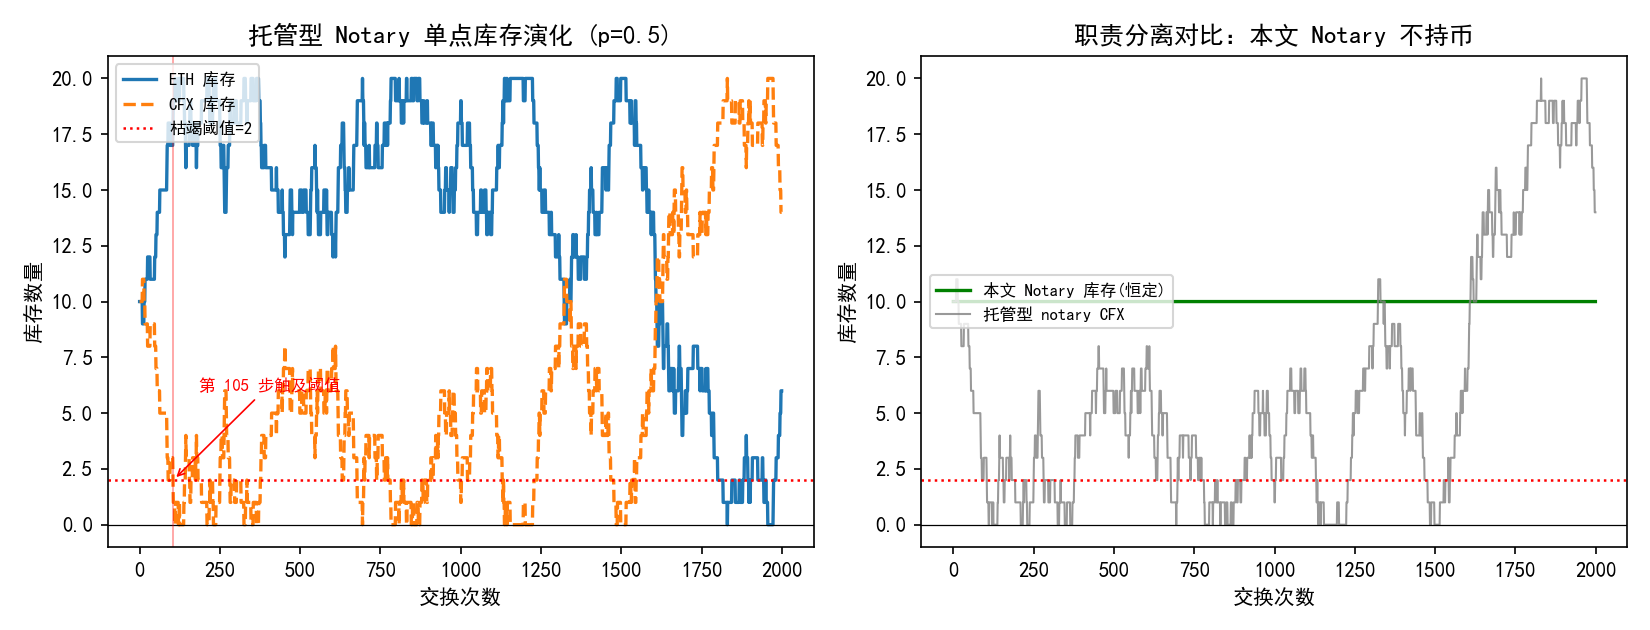
\includegraphics[width=0.95\textwidth]{figures/notary_liquidity_unbiased.png}
  \caption{无偏需求（$p=0.5$）下的库存演化。左图为一个代表性托管型 notary 的 ETH（实线）与 CFX（虚线）库存：每笔交换使一种币加一、另一种减一，库存随机漂移并在第 105 步触及阈值；右图将其与本文 Notary 的恒定库存对比}
  \label{fig:notary_unbiased}
\end{figure}

图~\ref{fig:notary_biased} 给出有偏需求（$p=0.7$，模拟单向跨链热点）的结果。左图同样以一个代表性 notary 展示：单向需求下其 CFX 库存被快速抽干、ETH 单向累积，第 80 步即触及阈值。从总体看枯竭显著加速，平均首次枯竭提前到第 106 步，末态各 notary 的 CFX 库存几乎归零而 ETH 大量累积，2000 笔交换中高达 809 笔（约 40\%）因目标链无货而被拒绝——这正对应\textquotedblleft 公证人最终只剩源链资产、却无法继续服务\textquotedblright 的失衡状态。与之相对，本文 Notary 在两种工况下库存始终恒定、拒绝交换数为零，不受流动性限制。

\begin{figure}[htbp]
  \centering
  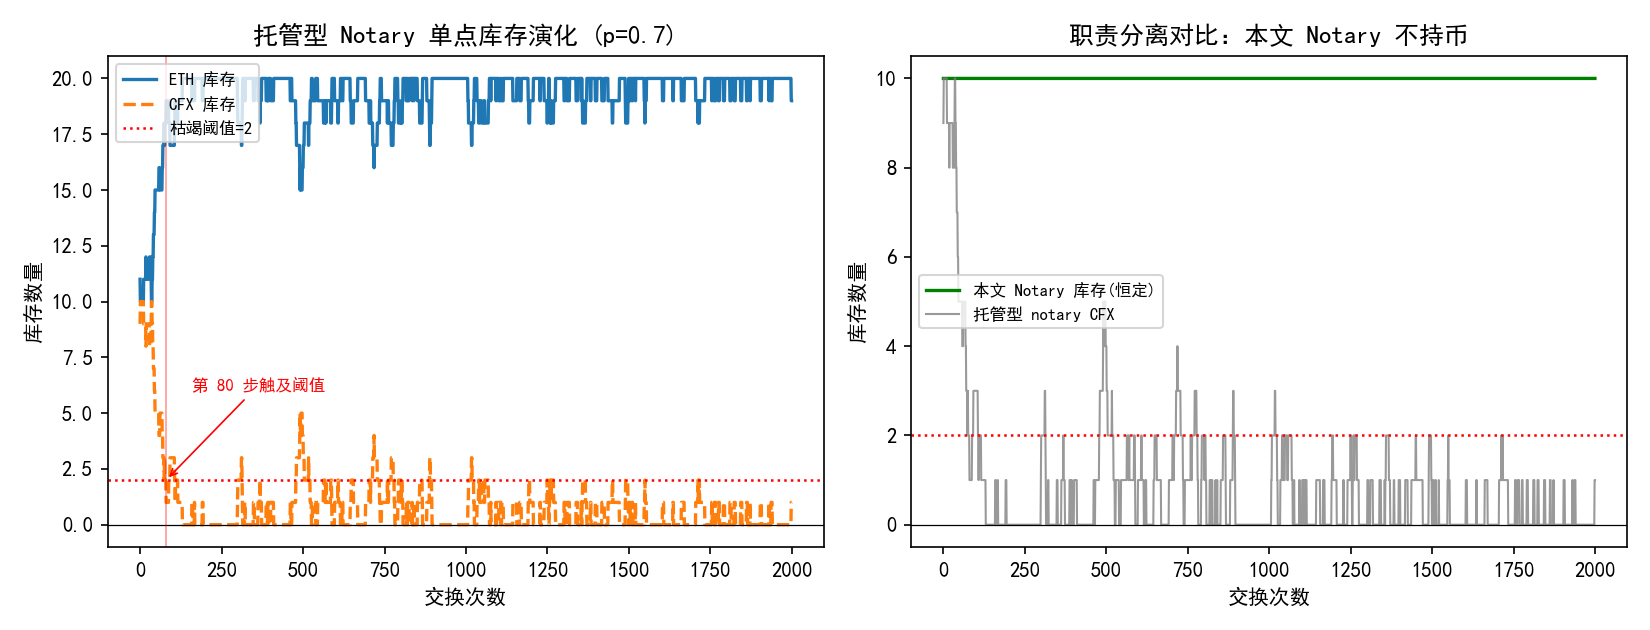
\includegraphics[width=0.95\textwidth]{figures/notary_liquidity_biased.png}
  \caption{有偏需求（$p=0.7$）下的库存演化。左图为一个代表性托管型 notary 的 ETH（实线）与 CFX（虚线）库存：单向需求下 CFX 快速耗尽、ETH 单向累积，第 80 步即触及阈值；右图与本文 Notary 的恒定库存对比}
  \label{fig:notary_biased}
\end{figure}

需要再次强调仿真的边界：该实验对象是 Notary 角色，结论为\textquotedblleft 托管型 notary 必然因库存失衡而枯竭，本文 Notary 因不持有资产而免疫\textquotedblright，并不代表本文系统整体不存在流动性问题——目标链 Manager 资金池在长期单向交换下同样会被耗尽。本文的价值在于将这一问题从消息中继职责中剥离，隔离到可独立治理的 Manager 角色，而非声称消除了它。

% !TEX root = ../main.tex

\chapter{系统实现与展示}


\section{智能合约实现}


智能合约模块是本文系统在合约链上的核心实现。\texttt{CrossChainTokenPool.sol} 同时承担资产池、跨链中间代币和 HTLC 状态机功能。合约的实现重点不是单次转账，而是维护跨链交换在不同阶段的状态：用户侧锁定由 \texttt{CrossChainSwap} 表示，目标侧响应锁定由 \texttt{ManagerLock} 表示。两个结构体的核心字段如下。


\begin{codeblock}[language=Solidity]
struct CrossChainSwap {
    bytes32 hashLock;
    uint256 timeLock;
    address sender;
    address recipient;
    uint256 amount;
    bool completed;
    bool refunded;
    bool isManagerLocked;
}

struct ManagerLock {
    bytes32 hashLock;
    uint256 timeLock;
    address recipient;
    uint256 amount;
    bool completed;
    bool refunded;
}
\end{codeblock}


其中，\texttt{hashLock} 用于约束领取条件，\texttt{timeLock} 用于约束退款条件，\texttt{completed} 和 \texttt{refunded} 用于避免同一笔交换重复完成或重复退款。用户发起跨链交换后，合约将资产转入合约地址并写入 \texttt{CrossChainSwap}；Notary 或目标侧执行节点响应后，合约创建 \texttt{ManagerLock}，使目标链资产与源链锁定通过同一个 \texttt{hashLock} 关联。


核心接口可以概括为以下几类。


\begin{codeblock}[language=Solidity]
function initiateCrossChain(
    bytes32 hashLock,
    address recipient,
    uint256 amount,
    uint256 timeLockBlocks
) external returns (bytes32 swapId);

function managerRespondToCrossChain(
    bytes32 hashLock,
    address recipient,
    uint256 amount,
    uint256 timeLockBlocks
) external;

function completeCrossChain(bytes32 swapId, bytes32 secret) external;
function completeManagerLock(bytes32 hashLock, bytes32 secret) external;

function refundCrossChain(bytes32 swapId) external;
function refundManagerLock(bytes32 hashLock) external;
\end{codeblock}


这些接口分别对应跨链流程中的发起、响应、完成和退款四个阶段。完成阶段的关键检查是 \texttt{keccak256(abi.encodePacked(secret)) == hashLock}，只有提交正确 secret 才能改变交易状态；退款阶段的关键检查是当前区块高度已经超过 \texttt{timeLock}，并且交易尚未完成。合约还通过 \texttt{CrossChainInitiated}、\texttt{CrossChainCompleted}、\texttt{ManagerLockCreated}、\texttt{ManagerLockCompleted}、\texttt{CrossChainRefunded} 和 \texttt{ManagerLockRefunded} 等事件向链下模块暴露状态变化。Notary 监听这些事件后即可驱动目标链执行对应操作。


\section{后端服务实现}


后端服务承担跨链协调职责，核心任务是将不同链之间无法直接通信的现实转化为统一的跨链状态管理。系统采用 Python Flask 框架，按照链类型划分为多个 coordinator 模块，每个 coordinator 封装对应链的节点连接、交易构造和事件解析逻辑。

后端的模块结构如下。顶层为统一的 API 路由层，负责接收前端或外部调用的跨链请求；中间层为 coordinator 分发层，根据请求中的 \texttt{sourceChain} 和 \texttt{targetChain} 字段将请求路由到对应的链处理模块；底层为各链适配模块，包括 ETH coordinator（通过 Web3.py 与 EVM 合约交互）、BSC coordinator（复用 EVM 适配逻辑但连接不同节点）、Conflux coordinator（通过 conflux-web3 适配）、Fabric coordinator（通过 SDK 调用链码）以及 BTC coordinator（作为无脚本链场景的替代实现，处理 adaptor signature 状态）。这种分层设计使得新增链适配只需实现底层模块，不影响上层路由和状态管理。

通用跨链接口包括：


\begin{codeblock}
POST /cross-chain/initiate
POST /cross-chain/complete/<swap_id>
POST /cross-chain/refund/<swap_id>
GET  /cross-chain/status/<swap_id>
GET  /cross-chain/active
\end{codeblock}


对于 BTC 适配场景，后端还提供独立入口：


\begin{codeblock}
POST /cross-chain/eth-to-btc/initiate
POST /cross-chain/eth-to-btc/complete/<hash_lock>
GET  /cross-chain/eth-to-btc/status/<hash_lock>
\end{codeblock}


在核心流程中，后端从交易回执中解析 \texttt{CrossChainInitiated} 事件，提取 \texttt{swapId}、\texttt{hashLock}、\texttt{amount}、\texttt{recipient} 和 \texttt{timeLock} 等参数，并根据目标链类型调用对应 coordinator 的响应方法。如果链上交易提交失败（如 gas 不足或网络超时），coordinator 会记录失败状态并暴露给前端，由用户决定是否重试或等待 timeLock 到期后退款。后端不会在链上交易失败时自动重试并提交新交易，以避免在不确定状态下造成重复锁定。

需要强调的是，后端服务并不是安全性的唯一来源。它可以帮助自动化流程、提高用户体验，但资产能否释放仍由合约或签名协议决定。即使后端出现异常，系统仍应依靠 timeLock 提供退款路径。这一点与第五章的 Notary 信任边界分析一致：后端与 Notary 更接近流程协调层，而不是最终资产安全的唯一保证。


\section{前端可视化实现}


前端模块服务于两个目的：一是提供跨链交换的产品原型入口，二是通过 HTLC 演示页面将协议流程可视化，辅助论文展示和系统验证。

跨链交换页面展示源链、目标链、跨链模式、接收地址和金额等输入项。该页面为纯前端原型，用于展示产品形态，不直接触发链上交易。用户提交表单后，前端调用后端 \texttt{/cross-chain/initiate} 接口，由后端完成实际的链上操作。

HTLC 演示页面是论文展示的核心组件。该页面围绕 Alice - ManagerA - Notary - ManagerB - Bob 五个角色展开，采用纯前端状态驱动的方式模拟协议执行过程，不依赖后端 API 或真实链上交易。用户通过”推进”按钮逐步触发状态转换，每一步对应协议中的一个阶段：生成 secret、计算 hashLock、源链锁定、Notary 监听、目标链响应、揭示 secret、Bob 领取或超时退款。前端状态模型如下。


\begin{codeblock}
interface HtlcDemoState {
  scenario: 'complete' | 'refund';
  currentStep: number;
  completed: boolean;
  refunded: boolean;
  secret: string;
  hashLock: string;
  timeLock: string;
  swapId: string;
  txHash: string;
}
\end{codeblock}


其中 \texttt{scenario} 区分正常完成路径和超时退款路径，\texttt{currentStep} 控制流程推进，页面右侧同步展示 \texttt{secret}、\texttt{hashLock}、\texttt{timeLock}、\texttt{swapId}、各角色余额变化和当前状态。这种纯前端模拟的设计选择是有意为之：它使演示不受链环境可用性的影响，能够在任何场景下稳定展示协议流程和安全条件，适合作为论文答辩和系统验证的辅助工具。


\section{实验流程设计}


为了验证系统功能和安全性，本文分别从功能正确性、安全约束和异构适配三个角度进行实验。合约链实验在本地 Hardhat 网络上执行，测试工具为 Hardhat、ethers.js 和 Chai，测试文件为 \filepath{test/HTLC.test.js}。实验中部署两个 \texttt{CrossChainTokenPool} 实例，分别模拟源链 ETH 池和目标链 BSC 池；测试账户包括 manager、Alice 和 Bob；Alice 与 manager 预先通过 \texttt{swapNativeForToken} 获得测试代币，实验金额设置为 200 至 500 个测试代币，\texttt{secret} 由 \texttt{ethers.randomBytes(32)} 生成，\texttt{hashLock} 由 \texttt{ethers.keccak256(secret)} 计算得到。无脚本链场景的 adaptor signature 实验在 Python 模拟环境中执行，测试文件为 \filepath{schnorr/test_scenario.py}，依赖 ECPy 椭圆曲线库，以 BTC 的 secp256k1 曲线作为替代实现。


\subsection{功能正确性验证}


功能正确性实验验证正常跨链路径是否能够完成。实验步骤为：Alice 在源链调用 \texttt{initiateCrossChain} 发起跨链请求，合约产生 \texttt{CrossChainInitiated} 事件；目标链执行 \texttt{managerRespondToCrossChain} 创建 \texttt{ManagerLock}；随后 Alice 调用 \texttt{completeCrossChain} 揭示 secret，Bob 使用同一 secret 调用 \texttt{completeManagerLock} 领取目标链资产。实际测试结果显示，交易依次触发 \texttt{CrossChainCompleted} 和 \texttt{ManagerLockCompleted} 事件，源链 \texttt{CrossChainSwap.completed} 与目标链 \texttt{ManagerLock.completed} 均变为 \texttt{true}，Bob 的目标链余额增加到测试设定的 \texttt{swapAmount}。该实验对应第五章的原子性分析，说明同一个 secret 能够联动两侧状态完成。


退款路径实验验证失败退出能力。实验中 Alice 发起跨链锁定后不公开 secret，测试脚本通过 Hardhat 时间辅助函数推进区块高度，使 timeLock 到期。随后 Alice 调用 \texttt{refundCrossChain}，manager 调用 \texttt{refundManagerLock}。实际结果显示，合约分别触发 \texttt{CrossChainRefunded} 和 \texttt{ManagerLockRefunded} 事件，Alice 与 manager 的测试代币余额恢复到初始水平。该结果对应第五章 5.1 中的可退款性说明，表明当 secret 未公开时，系统不会造成资金永久锁定。


\subsection{安全约束验证}


安全约束实验验证 hashLock 防护、权限控制、重复锁定防护和 timeLock 不对称约束。

重复 hashLock 实验中，manager 第一次使用某一 \texttt{hashLock} 创建 \texttt{ManagerLock} 后，再次使用同一 \texttt{hashLock} 创建锁定会被合约拒绝，revert 信息为 \texttt{Hash lock already used}。该结果说明合约能够限制同一哈希锁被重复响应，降低重放和重复领取风险。

权限控制实验中，非授权账户尝试调用 \texttt{managerRespondToCrossChain}，交易被合约回滚，revert 信息为 \texttt{Only notary can call this function}。该结果表明目标链响应动作受到角色权限限制，非授权地址无法触发关键状态变更，与第五章对 Notary 信任边界的分析相对应。

更新测试脚本中的权限命名后，Hardhat 输出显示 6 个测试用例全部通过，说明正常完成、超时退款、重复 hashLock 防护和非授权调用拒绝等约束均能在本地测试环境中得到验证。

错误 secret 实验中，调用 \texttt{completeCrossChain} 时提交一个与 \texttt{hashLock} 不匹配的 secret，合约执行 \texttt{keccak256(abi.encodePacked(secret)) == hashLock} 检查失败并回滚交易。该结果说明不知道正确 secret 的参与方无法完成领取，与第五章 5.1 的原子性约束相对应。

timeLock 不对称约束实验验证第五章 5.1 中论证的关键安全条件。实验设置源链 timeLock 为 100 个区块，目标链 ManagerLock 的 timeLock 为 50 个区块。测试脚本将区块高度推进至第 55 块（目标链 timeLock 已到期但源链 timeLock 未到期），此时目标链 \texttt{refundManagerLock} 可以成功执行，而源链 \texttt{refundCrossChain} 因 timeLock 未到期被拒绝。继续推进至第 105 块后，源链退款才可执行。该结果验证了 timeLock 不对称设置的正确性：目标链到期后源链仍有足够窗口供参与方使用 secret 完成结算，避免了双方同时退款导致原子性破坏的风险。


\subsection{异构适配验证}


无脚本链场景的 adaptor signature 实验验证机制流程。实验脚本依次生成 Alice、Bob、Carol 的 secp256k1 公私钥，构造聚合锁定点，生成 Alice 到 Bob 以及 Bob 到 Carol 的 adaptor signature。随后 Carol 补全签名并广播模拟交易，Bob 从该交易中提取秘密，再使用该秘密完成 Alice 到 Bob 的结算。整个流程仅使用签名生成、补全和验证操作，不依赖任何链上脚本，因此可直接迁移到 Monero、ZCash 屏蔽交易等无脚本链。实际运行输出显示：


\begin{codeblock}[extendedchars=true]
Tx_Bob_to_Carol confirmed on-chain.
Carol 成功领取资金。
Bob 从交易 Tx_Bob_to_Carol 中提取到了秘密。
Tx_Alice_to_Bob confirmed on-chain.
Bob 成功领取资金。
Simulation Complete.
\end{codeblock}


该实验说明在无脚本链场景中，交易完成与秘密提取之间能够建立联系。它对应第五章 5.4 的异构兼容分析：合约链通过 HTLC 在链上验证 secret，无脚本链通过签名补全关系暴露秘密，两者虽然实现方式不同，但都服务于“完成条件绑定”和“失败可退出”的安全目标。实验以 BTC 的 secp256k1 曲线作为替代实现，验证的机制不依赖脚本能力，可迁移到真正的无脚本链。


综上，第六章实验与第五章安全性分析形成对应关系：正常完成与退款实验验证 5.1 的原子性和可退款性；timeLock 不对称实验验证 5.1 中的时间约束安全条件；权限控制实验验证 5.2 的 Notary 信任边界；重复 hashLock 和错误 secret 实验验证 5.3 中对重放风险和 hashLock 防护的约束；adaptor signature 模拟实验验证 5.4 中多机制兼容的可行性。


\section{性能与代价评估}


在功能与安全验证之外，本节进一步评估系统在 HTLC 路径上的实际代价，包括本地环境下的 gas 与存储开销，以及真实测试网环境下的时间开销。需要说明的是，这些指标针对的是链上 HTLC 合约方案；adaptor signature 路径运行于纯密码学的无脚本链，不涉及 gas 与合约存储，其评估留待真实无脚本链接入后进行（见第七章）。

\subsection{gas 与存储代价}


gas 与存储实验在本地 Hardhat 网络上执行（测试文件 \filepath{test/gas-benchmark.test.js}），覆盖合约部署及一笔完整跨链交换涉及的全部操作，gas 数据从交易回执的 \texttt{gasUsed} 字段读取。结果如表~\ref{tab:gas-cost} 所示。

\begin{table}[htbp]
  \centering
  \caption{HTLC 路径各操作的 gas 消耗（本地 Hardhat）}
  \label{tab:gas-cost}
  \begin{tabular}{@{}lr@{}}
    \toprule
    操作 & gas 消耗 \\ \midrule
    部署合约（单条链池子） & 3\,696\,469 \\
    \texttt{swapNativeForToken}（原生币兑换中间代币） & 76\,135 \\
    \texttt{initiateCrossChain}（源链发起锁定） & 198\,149 \\
    \texttt{managerRespondToCrossChain}（目标链创建锁定） & 171\,690 \\
    \texttt{completeCrossChain}（源链结算） & 71\,453 \\
    \texttt{completeManagerLock}（目标链领取） & 84\,224 \\
    \texttt{refundCrossChain}（源链退款） & 64\,410 \\
    \texttt{refundManagerLock}（目标链退款） & 65\,925 \\
    \bottomrule
  \end{tabular}
\end{table}

从数据可见，合约部署是一次性的最大开销（约 370 万 gas）；运行期单笔操作中，写入新状态的操作（\texttt{initiateCrossChain}、\texttt{managerRespondToCrossChain}）gas 较高，因为它们首次写入 \texttt{CrossChainSwap} 与 \texttt{ManagerLock} 结构的多个存储槽；而完成与退款操作主要修改既有状态的标志位，gas 较低。一笔完整的双侧交换（发起、响应、两侧完成）链上 gas 合计约 52 万，处于普通 ERC20 多笔转账的量级，表明 HTLC 方案在合约链上的运行开销是可接受的。

在存储方面，每笔交换在源链创建一条 \texttt{CrossChainSwap} 记录，在目标链响应后创建一条 \texttt{ManagerLock} 记录。按结构体字段的存储槽布局估算，\texttt{CrossChainSwap} 约占 8 个存储槽，\texttt{ManagerLock} 约占 6 个，一笔完整的双侧交换约新增 14 个存储槽。由于每笔交换独立占用各自的 mapping 条目，链上持久化存储成本随交换数量\textbf{线性增长}，主要来自 \texttt{crossChainSwaps} 与 \texttt{managerLocks} 两个 mapping。这一增长特性提示：在长期运行的部署中，已完成或已退款的历史记录可考虑通过清理或归档机制回收存储，以控制状态膨胀。

\subsection{真实测试网时间代价}


为评估系统在真实异构链环境下的时间开销，本文在 Sepolia（源链）与 Conflux eSpace 测试网（目标链）上部署合约并执行一次完整的跨链交换（脚本 \filepath{scripts/eth_cfx/timing-benchmark.js}）。实验采用职责分离的三方角色：Alice 在 Sepolia 发起、Notary/Manager 在 CFX 响应、Bob 在 CFX 领取、Alice 在 Sepolia 完成结算。完整路径与各阶段确认时间如表~\ref{tab:timing-cost} 所示。

\begin{table}[htbp]
  \centering
  \caption{Sepolia $\rightarrow$ CFX eSpace 跨链各阶段确认时间}
  \label{tab:timing-cost}
  \begin{tabular}{@{}lr@{}}
    \toprule
    阶段 & 确认时间 \\ \midrule
    Sepolia 源链发起确认（兑换并发起锁定） & 21.17\,s \\
    CFX 目标链响应确认（创建 ManagerLock） & 10.99\,s \\
    CFX Bob 领取确认（揭示 secret） & 9.09\,s \\
    Sepolia 源链完成确认（结算） & 13.22\,s \\ \midrule
    端到端总耗时 & 54.48\,s \\
    \bottomrule
  \end{tabular}
\end{table}

从结果看，一次完整跨链交换的端到端耗时约 54 秒，主要由四次链上交易的确认时间累加而成。其中 Sepolia 侧确认较慢（发起 21 秒、完成 13 秒），CFX eSpace 侧较快（响应 11 秒、领取 9 秒），差异来自两条链不同的出块速度和确认机制，公共 RPC 节点的网络延迟也有一定贡献。需要说明的是，本实验为单次真实运行的记录，具体数值会随测试网负载和 RPC 状态波动，此处用于说明数量级而非精确基准。

更值得关注的是 Notary 的活跃时长与成本。从脚本侧解析源链事件到向目标链提交响应交易，观测延迟仅约 13\,ms，说明协调逻辑本身开销极小；端到端时间几乎全部消耗在链上确认等待上。据此可量化 Notary 的活跃窗口：

\begin{itemize}
  \item \textbf{狭义活跃时长} $T_{\text{active}}$（从监听到源链事件到目标链 ManagerLock 创建确认）：约 \textbf{10.99\,s}；
  \item \textbf{广义活跃时长}（从监听到源链事件到目标链领取完成）：约 \textbf{20.08\,s}；
  \item Notary 在目标链发起响应交易的 gas 消耗：291\,678。
\end{itemize}

这组数据为第五章 5.5 节的论证提供了真实环境的量化注脚：Notary 的成本表现为\textbf{一段以秒计的在线活跃窗口加上一笔目标链响应的 gas}，而非任何形式的资本占用。它在整个跨链过程中既不接收源链资产，也不垫付目标链流动性，目标链资产由 Manager 资金池提供。这与传统资金托管型公证人形成鲜明对比——后者必须预先准备并持续再平衡两条链的库存。由此，运行一个 Notary 节点的门槛被压低为\textquotedblleft 在线 + gas\textquotedblright，首个中继节点即可零资本接入。

% !TEX root = ../main.tex

\chapter{总结与展望}


\section{工作总结}


本文围绕跨链资产交换问题，设计并实现了一个基于公证人协调与哈希时间锁的原型系统。系统采用 Alice - ManagerA - Notary - ManagerB - Bob 的角色模型，将跨链流程抽象为用户请求、资金池锁定、公证中继、目标链响应和资产释放之间的协作关系，使各环节的控制边界清晰可分析。在机制层面，系统针对不同链的脚本表达能力提供了两种条件锁定方式：对于 EVM 类合约链，通过链上 HTLC 状态机实现 hashLock 条件领取和 timeLock 超时退款；对于 Monero、ZCash 屏蔽交易等无脚本链，由于 HTLC 的条件分支无法在链上表达，系统通过 Schnorr adaptor signature 将条件锁定放入签名补全过程，使仅具备签名能力的链也能参与原子交换。在安全性分析层面，本文针对 Notary 和 Manager 分别建立攻击模型，论证了系统在拒绝服务、参数篡改、重放攻击、抢跑攻击和密钥泄露等场景下的防御能力，并分析了两种机制在原子性保证上的安全等价性和跨机制秘密传递的正确性条件。在工程实现层面，项目完成了 Solidity 智能合约、Python 后端协调服务、scriptless 场景的 adaptor signature 模拟模块（以 BTC 作为替代实现）和前端可视化页面的组合：在本地 Hardhat 环境验证了功能正确性、安全约束、异构适配以及 gas 与存储代价，并在 Sepolia 与 Conflux eSpace 测试网上完成了真实环境的端到端跨链交换，测得各阶段确认时间、端到端耗时与 Notary 活跃时长。


\section{系统不足}


鉴于时间上的客观原因，项目在原型实现的真实性上留有遗憾。首先，无脚本链适配模块以机制模拟为主，目前以 BTC 的 secp256k1 曲线作为替代实现，尚未接入 Monero、ZCash 等真实无脚本链的交易流程，adaptor signature 的正确性仅在本地 Python 环境中验证。其次，Notary 当前更接近单节点协调模型，虽然合约和 timeLock 可以限制其直接资产风险，但其可用性仍可能影响跨链体验。再次，Manager 资金池的流动性管理较为简单，尚未充分考虑复杂汇率、手续费、滑点、限额和风险控制。此外，测试网时间代价实验仅为单次真实运行的记录，受公共 RPC 与测试网负载影响，尚缺乏多轮、多负载条件下的统计基准。最后，系统安全性主要通过攻击模型分析和实验验证说明，尚未进行形式化证明和完整安全审计。


\section{后续展望}


后续工作可以围绕安全性增强、真实环境接入和系统能力扩展三个方向推进。

在安全性增强方面，当前 Notary 为单节点协调模式，后续可以引入多 Notary 节点，通过多签触发或门限签名机制使跨链消息转发不再依赖单一节点的可用性。同时，HTLC 与 adaptor signature 的安全性可以通过形式化建模进一步论证，从而更严格地分析系统在延迟、抢跑、节点失效和参数错配等攻击场景下的安全边界。

在真实环境接入方面，无脚本链适配模块需要从本地模拟扩展到真实链的交易流程，将 adaptor signature 应用于 Monero 或 ZCash 屏蔽交易等真实无脚本链的签名与花费过程。合约链侧已在 Sepolia 与 Conflux eSpace 测试网完成单次端到端验证，后续需扩大到多轮、多负载条件下的统计测量，以给出更稳健的确认延迟、gas 消耗与 Notary 活跃时长基准，并评估不同 timeLock 参数设置的合理性。

在系统能力扩展方面，Manager 资金池可以加入流动性监控、动态费率、额度限制和异常告警机制，以提高系统面对不同交易规模和市场波动时的稳定性。随着 Solana、Cosmos 等更多异构链的接入需求出现，系统还需要进一步抽象链适配接口，使不同交易模型的链能够以统一方式接入跨链协调层。

总体而言，本文系统展示了一种将公证人协调、HTLC 哈希时间锁和 Schnorr adaptor signature 结合起来的跨链资产交换方案。该方案的核心思路是：在架构层通过统一角色流程保持跨链协作的一致性，在机制层根据目标链的脚本表达能力选择适合的条件锁定方式，在安全层通过密码学绑定和超时退出保证原子性和可退款性。借助 adaptor signature 将条件锁定移出脚本层，该方案能够把原子交换的适用范围从智能合约链扩展到无脚本链，为异构区块链之间的资产互操作提供有价值的原型参考。


%TC:ignore

% 参考文献
\printbibliography[heading=bibintoc]

% 附录、致谢、成果和简历可在定稿阶段按学校要求补充。

%TC:endignore

\end{document}
